\chapter{Mechanische Modellbildung}
% todo Bild HMI Roboterkoordinaten ablesen
%
Gegenstand der Modellbildung ist die Definition von Bewegungsgleichungen zur Simulationen der Roboterdynamik \cite[S.~247]{Grimble.2009}. Damit soll die aufgenommene Energie des Roboters entlang einer Bewegungsbahnen bestimmt werden, ohne dass das reale System angesteuert werden muss. Zunächst erfolgt eine Beschreibung der Vorwärtskinematik mithilfe der Denavit-Hartenberg (DH) Konvention. Nach einer Betrachtung der Geschwindigkeits-Kinematik wird die inverse Dynamik des Systems beschrieben.  Abschließend wird der Wahrheitsgehalt des Modells überprüft.

\section{Vorwärtskinematik}
Über die Vorwärtskinematik erfolgt eine geometrische Beschreibung der Endeffektor Bewegung des Roboters entlang der kinematischen Kette \footnote{siehe Anhang \ref{add:kinematische-kette}}. Entsprechend der Gelenkvariablen wird dabei die Position und Orientierung (Pose) des Endeffektors im Basis-Koordinatensystem berechnet. Ausgehend vom Basis-Koordinatensystem werden homogene Transformationsmatrizen $\bm{A}(i) = \bm{T}^{i-1}_i \in \text{SE(3)}$\footnote{siehe Anhang \ref{add:SE3}} zwischen zwei aufeinanderfolgenden Koordinatensystemen $0_{i-1}x_{i-1}y_{i-1}z_{i-1}$ und $0_ix_iy_iz_i$ der kinematischen Kette definiert. $\bm{T}^{i-1}_i$ repräsentiert die  Rotation und Translation des KS$\left\{i\right\}$ im $\left\{i-1\right\}$. Die Transformationsmatrizen sind abhängig von der Konfiguration der Gelenkvariablen $q_i$ des Roboters. 
\begin{align}
	\bm{A}_i = \bm{A}_i(q_i)
\end{align}
Eine Repräsentation der Endeffektor-Pose $H$ im Basis-Koordinatensystem wird über eine Multiplikation der homogenen Transformationsmatrizen entlang der kinematischen Kette erreicht. 
\begin{align}
	\label{eqn:homogeneTransformation}
	\bm{H} = \bm{T}^0_n = \bm{A}_1(q_1) ... \bm{A}_n(q_n)
\end{align}
\begin{align}
	\bm{H} =\begin{bmatrix} \bm{R}^0_n &\quad \bm{o}^0_n\\ \mathbf{0}_{1x3} &\quad 1\end{bmatrix}
\end{align}
Der Spaltenvektor $\bm{o}^0_n$ repräsentiert die Koordinaten des Ursprungs des Endeffektor-Koordinatensystems im Basis-Koordinatensystem. Die $3 \times 3 $ Matrix $\bm{R}^n_0$ entspricht der Rotation des Endeffektor-Koordinatensystems gegenüber dem Basis-Koordinatensystem. \cite[S.~75~ff.]{Spong.2020} 
%
\section{Denavit-Hartenberg Konvention}
Eine Methode zur Bestimmung der homogenen Transformationsmatrizen ist die, nach  dem Physiker Jacques Denavit und dem Ingenieur Richard Hartenberg benannte Denavit-Hartenberg Konvention. Diese besagt, dass jede homogene Transformation $\bm{A}_i$ als Produkt vier nacheinander ausgeführter elementarer Transformationen ausgedrückt werden kann. 
\begin{align}
	\label{eqn:elementarTransformation}
	A_i &= \text{Rot}_{z,\theta_i}\text{Trans}_{z,d_i}\text{Trans}_{x,a_i}\text{Rot}_{x,\alpha_i} \\
	&= \left[\begin{matrix}
		c_{\theta_i} &\quad -s_{\theta_i} &\quad 0 &\quad 0 \\
		s_{\theta_i} &\quad c_{\theta_i} &\quad 0 &\quad 0 \\
		0 &\quad 0 &\quad 1 &\quad 0 &\quad \\ 
		0 &\quad 0 &\quad 0 &\quad 1 &\quad 
	\end{matrix}\right] 
	\left[\begin{matrix}
		1 &\quad 0 &\quad 0 &\quad 0 \\
		0 &\quad 1 &\quad 0 &\quad 0 \\
		0 &\quad 0 &\quad 1 &\quad d_i &\quad \\ 
		0 &\quad 0 &\quad 0 &\quad 1 &\quad 
	\end{matrix}\right] \notag \\
	& \times
	\left[\begin{matrix}
		1 &\quad 0 &\quad 0 &\quad a_i \\
		0 &\quad c_{\alpha_i} &\quad -s_{\alpha_i} &\quad 0 \\
		0 &\quad s_{\alpha_i} &\quad c_{\alpha_i} &\quad 0 &\quad \\ 
		0 &\quad 0 &\quad 0 &\quad 1 &\quad 
	\end{matrix}\right]
	\left[\begin{matrix}
		1 &\quad 0 &\quad 0 &\quad 0 \\
		0 &\quad 1 &\quad 0 &\quad 0 \\
		0 &\quad 0 &\quad 1 &\quad 0 &\quad \\ 
		0 &\quad 0 &\quad 0 &\quad 1 &\quad 
	\end{matrix}\right]
	\notag \\
	c = cos\notag \\
	s = sin \notag 
\end{align}
Die Parameter entsprechen dem Gelenkwinkel $\theta_i$, dem Gelenkabstand $d_i$, der Armelementlänge $a_i$ und der Verwindung $alpha_i$, wobei $d_i$, $a_i$ und $alpha_i$ konstant sind. \cite[S.~79]{Spong.2020}
%
\subsection*{Festlegung der Koordinatensysteme}
Abbildung \ref{fig:kr210} zeigt den zu untersuchenden KUKA KR210 R2700-2 Industrieroboter. Die Bezeichnung der Maschine gibt Auskunft über ihre technischen Daten.  Die Nenn-Traglast beträgt 210 kg. Die maximale Reichweite des Roboters liegt bei 2701 mm. Weitere Informationen sind dem Datenblatt, siehe Anhang \ref{add:datenblatt} zu entnehmen.  
%
\begin{figure}[tbph]
	\centering
	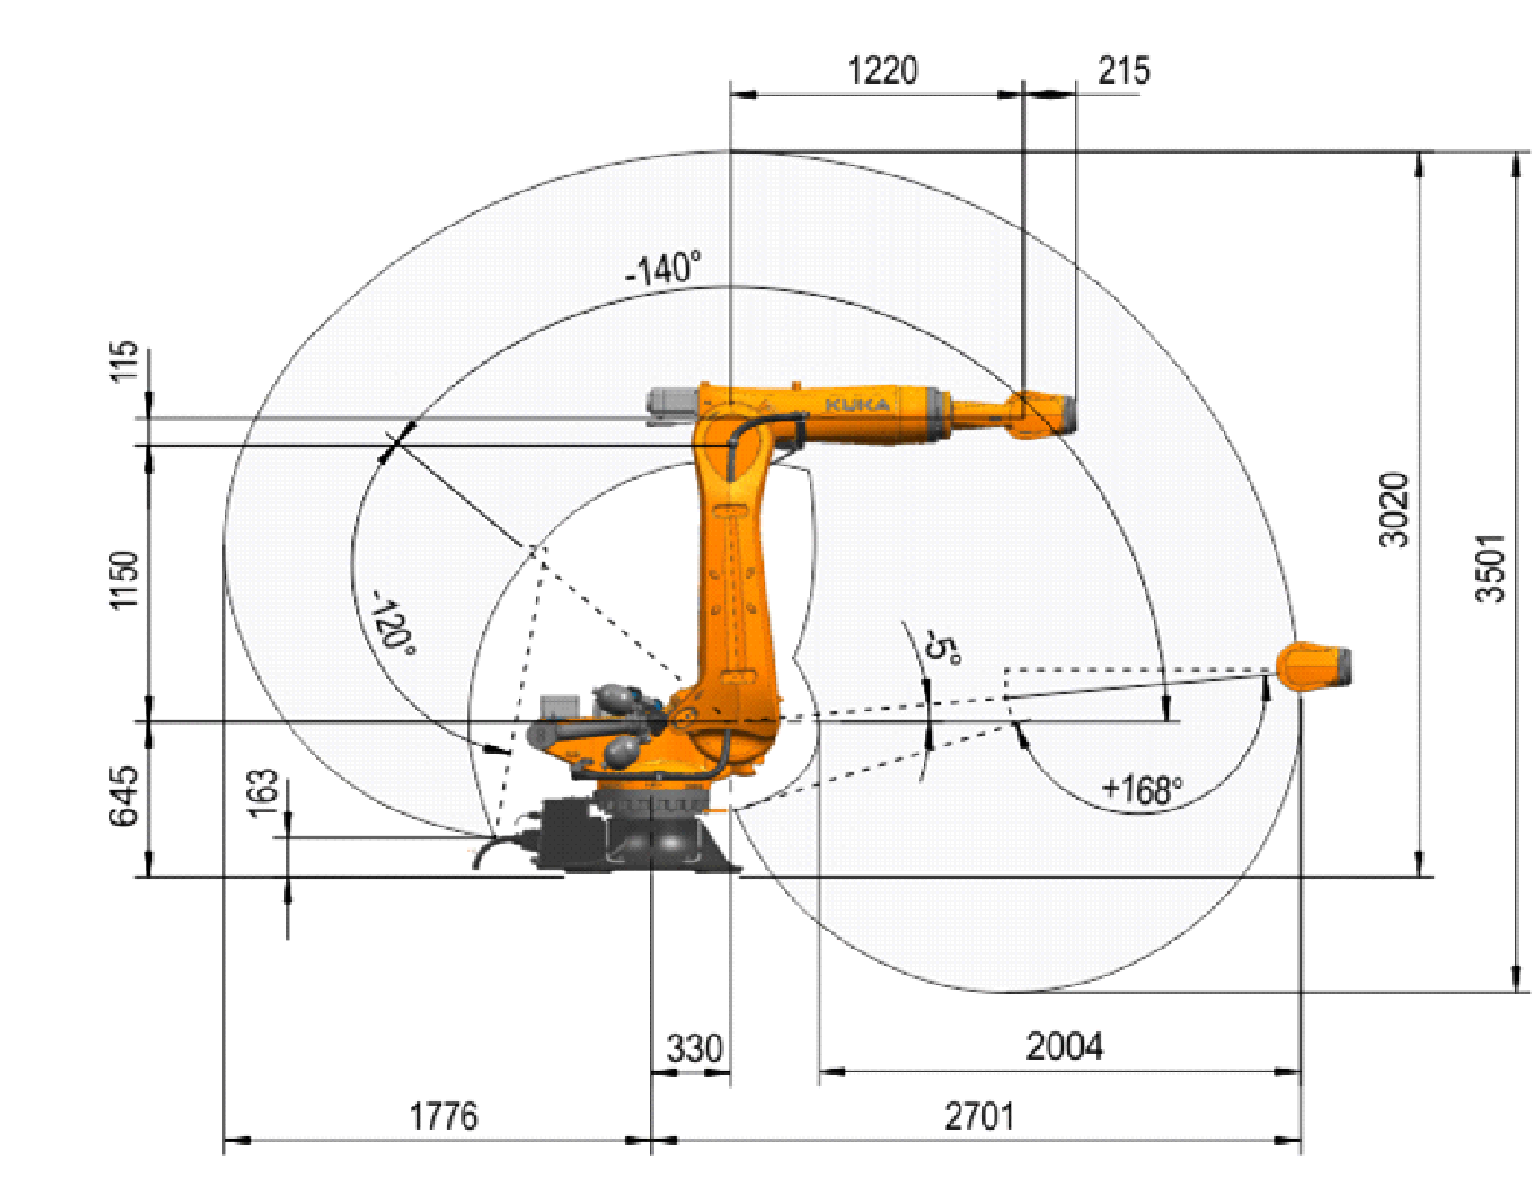
\includegraphics[width=0.8\linewidth]{images/KR210}
	\caption{KUKA KR210 R2700-2}
	\label{fig:kr210}
\end{figure}
%
Im ersten Schritt werden die Achsen $z_i, \ i = 0,...,n-1, n=6$, siehe Abbildung \ref{fig:zachsen} definiert. Im zweiten Schritt wird das Basiskoordinatensystem ${0}$ definiert, wobei der Ursprung $\bm{o}_0$ auf der Achse $z_0$ platziert wird. Die Definition des ersten Koordinatensystems entspricht dem ROBROOT-Koordinatensystem, welches vom Hersteller auf der Robotersteuerung hinterlegt ist. Diese Festlegung erlaubt eine Überprüfung der Vorwärtskinematik mithilfe der, von der KUKA Robotersteuerung (Robot Control (KR C)) berechneten kartesischen Koordinaten. Des Weiteren werden, siehe Abbildung \ref{fig:KS} aufsteigend die Koordinatensysteme KS$\{i\},i=1,...,n-1$ basierend auf KS$\left\{i-1\right\}$, sowie das rot hervorgehobene Endeffektor-Koordinatensystem $0_6x_6y_6z_6$ platziert. Es werden folgende Regeln berücksichtigt.  
%
\begin{figure}[tbph]
	\centering
	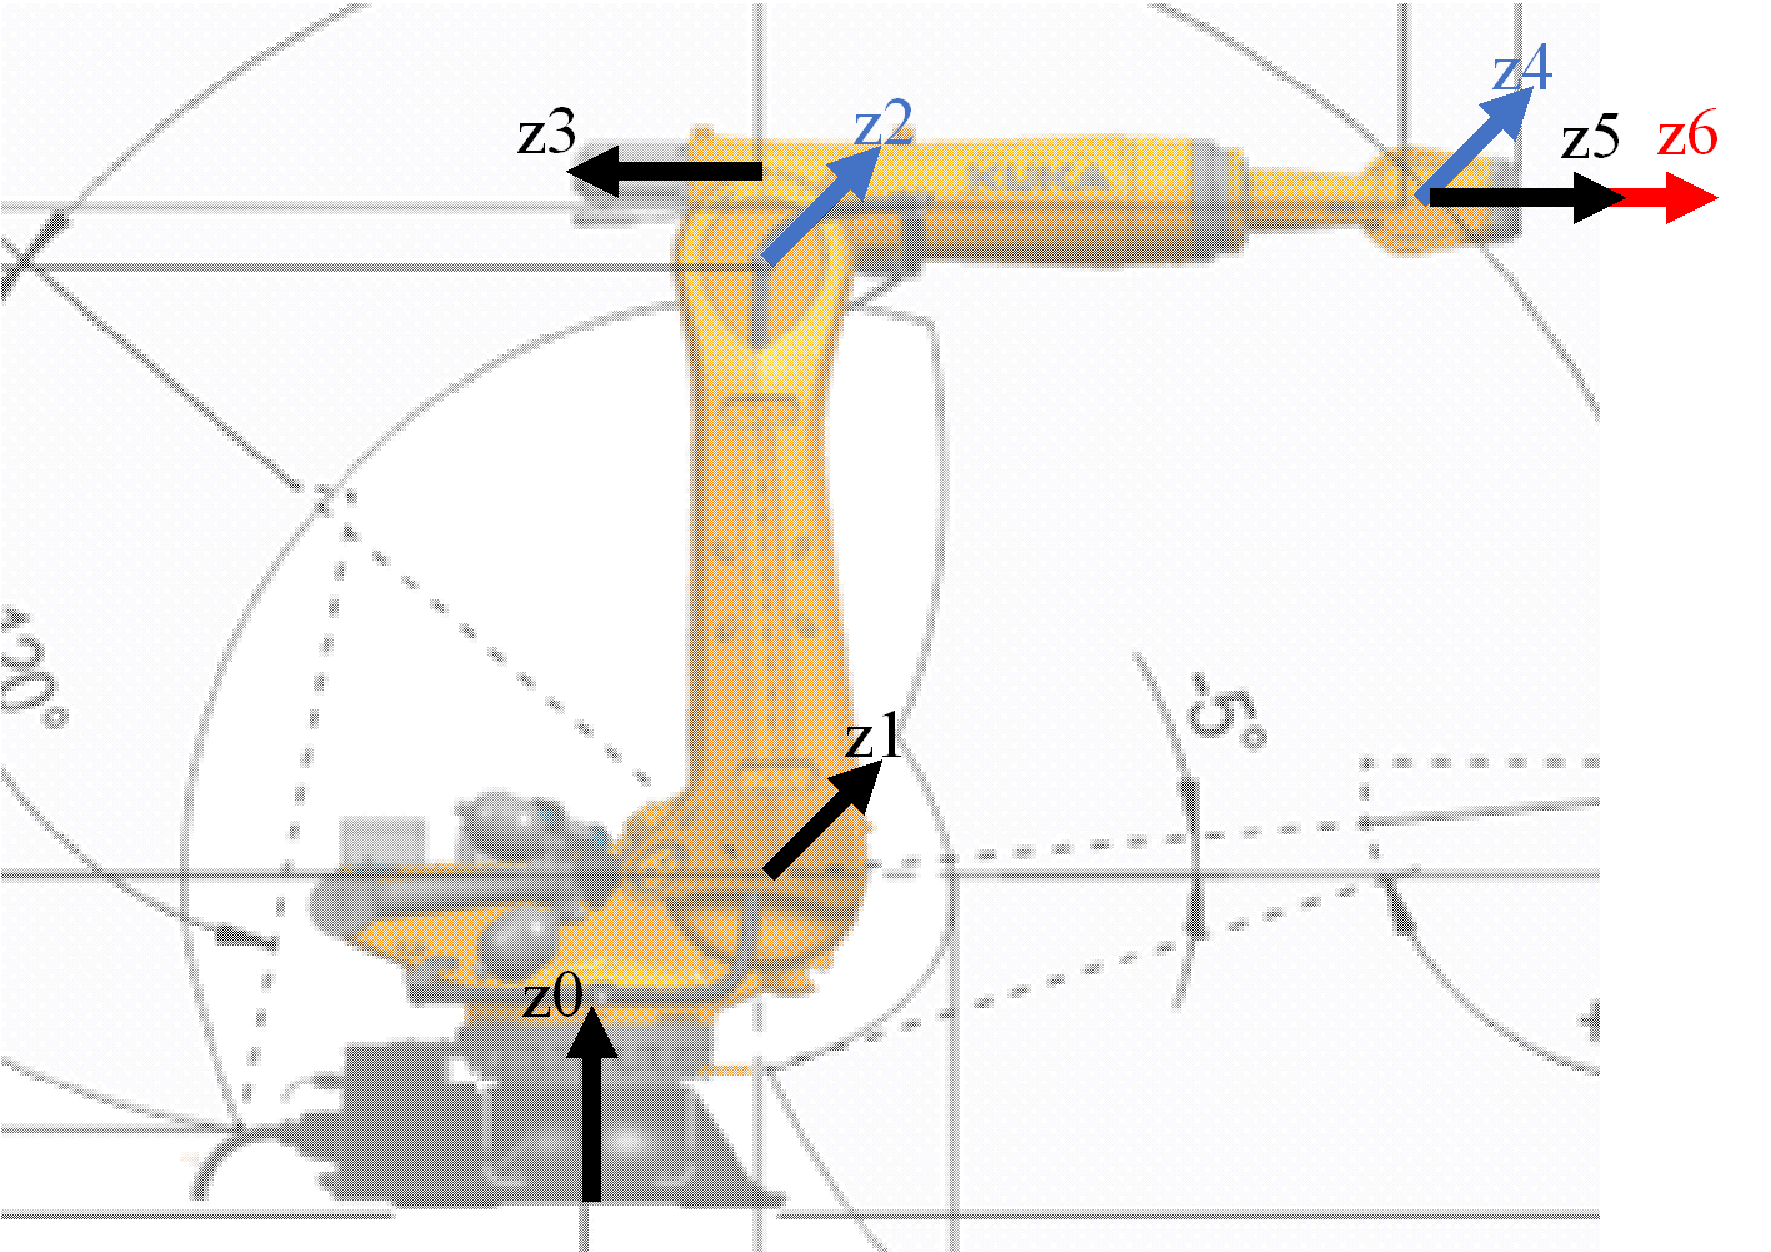
\includegraphics[width=0.5\linewidth]{images/zAchsen}
	\caption[]{Festlegung der z-Achsen}
	\label{fig:zachsen}
\end{figure}
%
\begin{figure}[tbph]
	\centering
	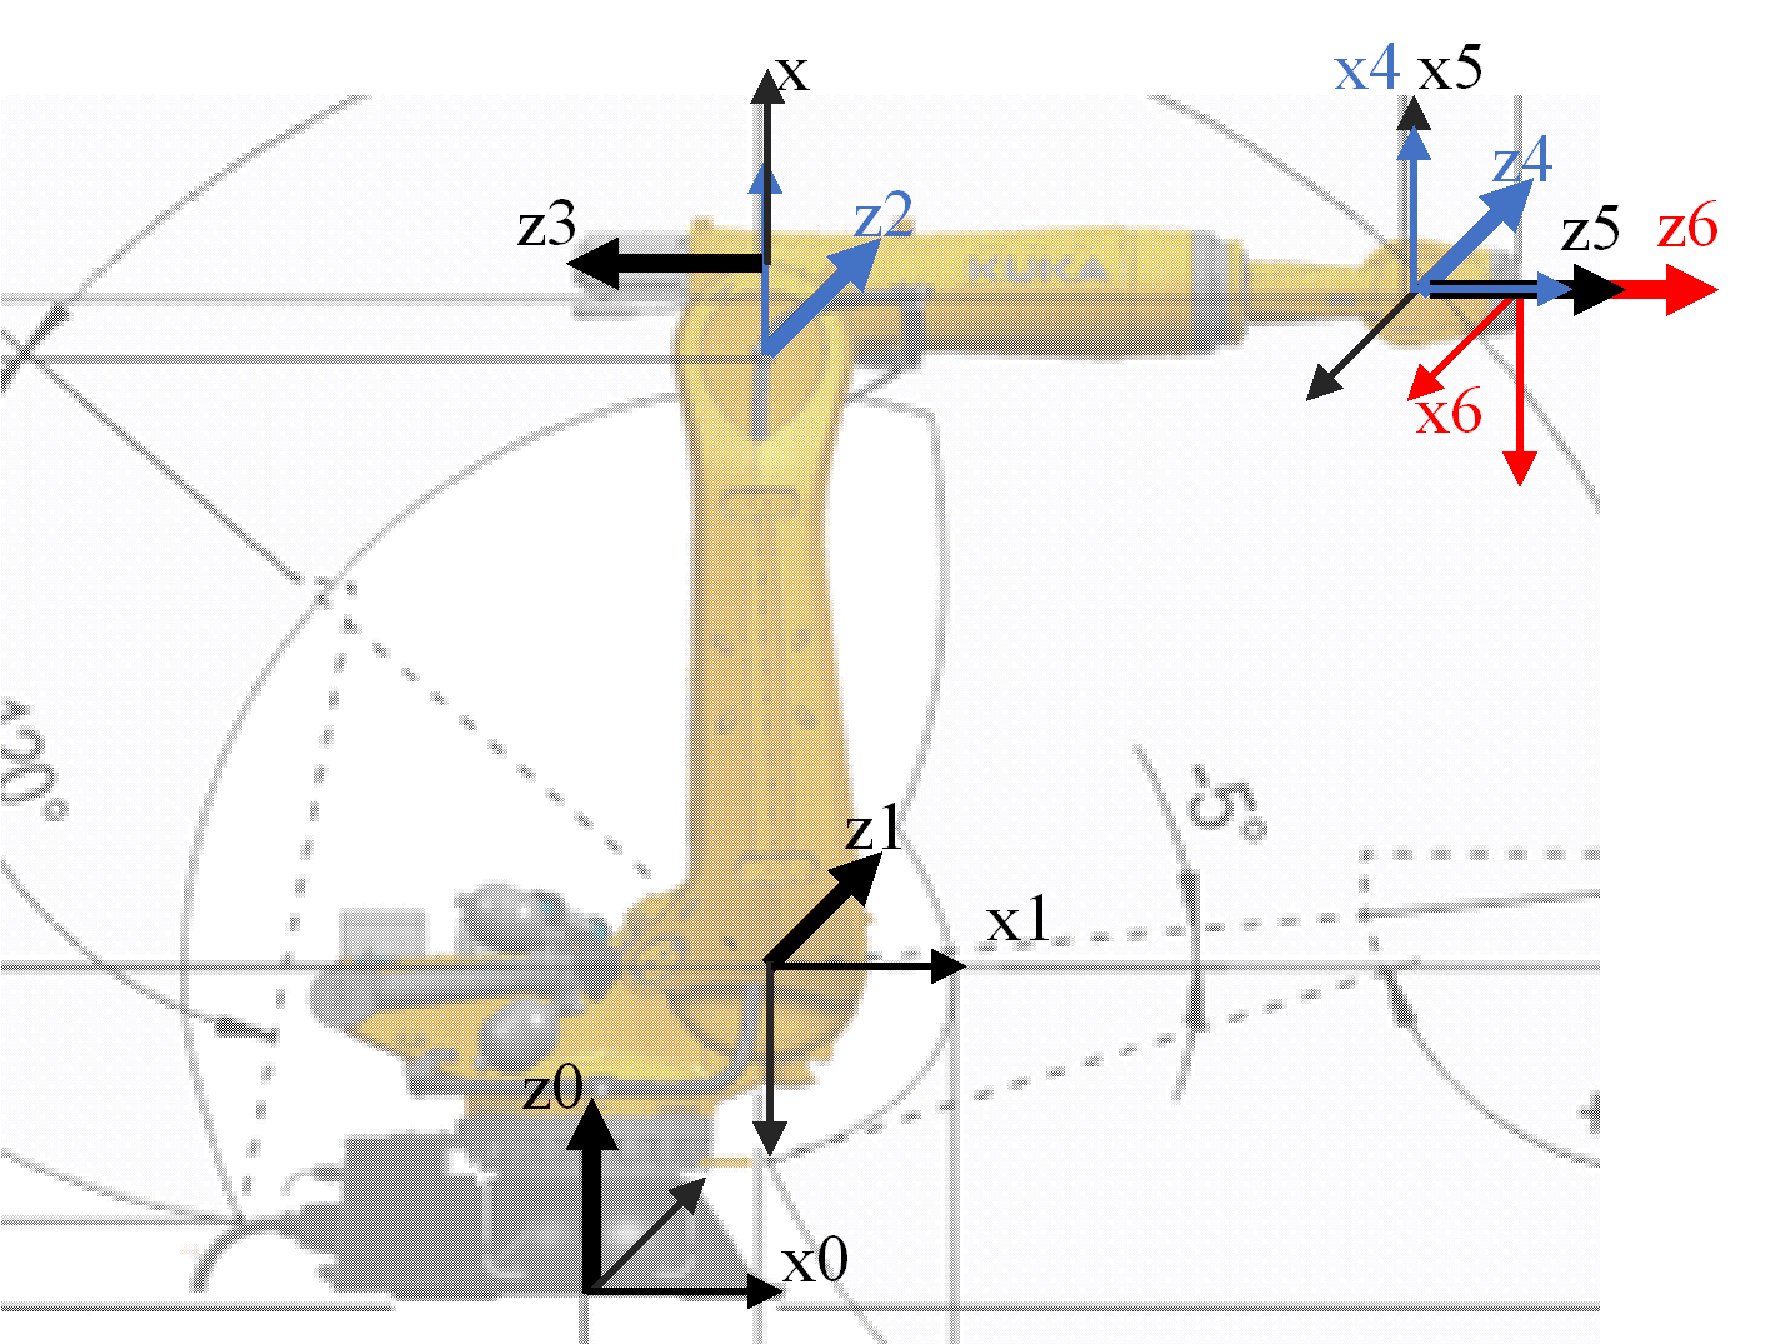
\includegraphics[width=0.5\linewidth]{images/KS}
	\caption{Festlegung der Koordinatensysteme}
	\label{fig:KS}
\end{figure}
%
\begin{itemize}
	\item Falls sich $z_i$ und $z_{i-1}$ scheiden, ist der Ursprung $\bm{o}_i$ in den Schnittpunkt zu legen. Die Achse $x_i$ wird rechtwinklig zur $z_{i-1}-z_i$-Ebene definiert. (gilt für KS$\left\{4\right\}$ und KS$\left\{5\right\}$)
	\item Falls  $z_i$ und $z_{i-1}$ parallel sind, wird der Ursprung $\bm{o}_i$ auf die Achse $z_i$ gelegt. Die Achse $x_i$ wird parallel zur gemeinsamen Normale von $z_i$ und $z_{i-1}$	im Punkt $\bm{o}_i$ definiert. (gilt für KS$\left\{2\right\}$)
	\item Falls  $z_i$ und $z_{i-1}$ nicht koplanar sind, wird der Ursprung $\bm{o}_i$ auf den Schnittpunkt der Achse $z_i$ mit der gemeinsamen Normalen von $z_i$ und $z_{i-1}$  gelegt. Die Achse $x_i$ ist die gemeinsamen Normale von $z_i$ und $z_{i-1}$. (gilt für KS$\left\{1\right\}$ und KS$\left\{3\right\}$)
	\item die Achse $y_i$ vervollständigt das rechtshändige, kartesische Koordinatensystem
\end{itemize} 
%
Im nächsten Schritt werden DH-Parameter, identifiziert.  $\theta_i$ entspricht der Rotation um $z_{i-1}$, sodass $x_{i-1}||x_i$. Der Parameter $d_i$ drückt die Translation entlang $z_{i_1}$ bis zum Schnittpunkt S von $z_{i-1}$ und $x_i$ aus. Der Parameter $a_i$ entspricht der Translation entlang $x_i$, um den Schnittpunkt S in den Ursprung $o_i$ zu überführen. $\alpha_i$ ist die Rotation um $x_i$, sodass $z_{i-1}$ in $z_i$ überführt wird. Aus den Elementartransformationen, siehe Gleichung \ref{eqn:elementarTransformation} wird die Gesamttransformationen entsprechend der Gleichung \ref{eqn:homogeneTransformation} berechnet. Tabelle \ref{tab:dh} listet die identifizierten DH-Parameter. 
%
\begin{table}[tbph]
	\centering
	\caption{Denavit-Hartenberg Parameter}
	\label{tab:dh}
	\begin{tabular}{|c|c|c|c|c|}
		\hline
		Gelenk & theta & d [m] & a [m] & alpha \\
		\hline
		1& 0 & 0,645 & 0,330 & $-90^\circ$ \\
		\hline
		2& $-90^\circ$ & 0 & 1,150 & 0 \\
		\hline
		3& 0 & 0 & 0,115 & $90^\circ$ \\
		\hline
		4& 0 & -1,220 & 0 & $-90^\circ$ \\
		\hline
		5& 0 & 0 & 0 & $-90^\circ$ \\
		\hline
		6& $90^\circ$ & 0,215 & 0 & 0 \\
		\hline
	\end{tabular}
\end{table}
%
Eine Verarbeitung der Gelenkwinkel, welche in der KR C für eine bestimmte Pose definiert sind, bedingt eine Anpassung DH-Parameter. Der Lieferant KUKA definiert die Achse $z_{1}$ um 180° rotiert ggü. der o. g. Festlegung. Folglich werden die, in der Robotersteuerung gegebenen Winkel des ersten Gelenks  mit -1 multipliziert, bevor eine Weiterverarbeitung im Modell erfolgt. Des Weiteren werden vom dritten Winkel 90° subtrahiert, bevor der Wert dem Modell übergeben wird. Die Vorwärtskinematik ist über drei verschiedene Posen am realen System verifiziert. Dabei ist festzustellen, dass in der Robotersteuerung die Biegung der Glieder berücksichtigt wird, wohingegen in der oben gezeigten Definition von einem Starrkörper-Modell ausgegangen wird. 
Die Implementierung der DH-Transformation ist im Anhang \ref{add:dh}  aufgeführt. 
%
\section{Geschwindigkeits-Kinematik}
Die Geschwindigkeits-Kinematik definiert die lineare Endeffektor-Geschwindigkeit, sowie die  Endeffektor-Winkelgeschwindigkeit in Abh{\"a}ngigkeit der Gelenkwinkelgeschwindigkeiten des Roboters. Eine mathematische Beschreibung des Zusammenhangs erfolgt {\"u}ber die Jacobi-Matrix der Vorw{\"a}rtskinematik \cite[S.~101]{Spong.2020}. Grundlegende Definitionen zur Aufstellung der Jacobi-Matrizen werden in \ref{add:geschwindigkeitskinematik} betrachtet. 
\subsection{Jacobi-Matrizen}
Die lineare Geschwindigkeit $\bm{v}^0_n$ des Endeffektors, sowie seine Winkelgeschwindigkeit $\bm{\omega}^0_{0,i}$ im  KS$\left\{0\right\}$ lassen sich über die $3\times n$-Jacobi-Matrizen $\bm{J}_v$ und $\bm{J}_{\omega}$ berechnen. 
%
\begin{equation}
	\bm{v}^0_n = \bm{J}_v \dot{\bm{q}} = \left[\bm{J}_{v1 \ \bm{J}_{v2}} \ ...\  \bm{J}_{vn}\right] \dot{\bm{q}}
\end{equation}
%
\begin{equation}
	\bm{\omega}^0_{0,i} = \bm{J}_{\omega} \dot{\bm{q}}  = \left[\bm{J}_{\omega1 \ \bm{J}_{\omega2}} \ ...\  \bm{J}_{\omega n}\right] \dot{\bm{q}}
\end{equation}
%
\begin{equation}
	\bm{J}_{vi} = \begin{cases} 
		\bm{z}^0_{i-1} \times (\bm{o}^0_{n} - \bm{o}^0_{i-1}) & \text{falls Gelenk } i \text{ vom Typ } \text{R} \\
		\bm{z}^0_{i-1} & \text{falls Gelenk } i \text{ vom Typ } \text{T}
	\end{cases}
\end{equation}
%
\begin{equation}
	\bm{J}_{\omega i} = \begin{cases} 
		\bm{z}^0_{i-1} = \bm{R}^0_{i-1}\bm{e}_3 & \text{falls Gelenk } i \text{ vom Typ } \text{R} \\
		\mathbf{0}_{3 \times 1} & \text{falls Gelenk } i \text{ vom Typ } \text{T}
	\end{cases}
\end{equation}
%
\begin{itemize}
	\item Ein Gelenk vom Typ R ist ein Rotationsgelenk.
	\item Ein Gelenk vom Typ T ist ein Translationsgelenk.
\end{itemize}
%
\cite{Rieber.2022}
%
% todo Relevanz Geeschwindigkeitskinematik
%
\section{Dynamik}
Ziel des Kapitels ist die Berechnung der aufzubringenden Momente in den sechs Gelenken des Roboters bei Ansteuerung entlang einer Bewegungsbahn.
Die Bewegungsgleichungen werden zunächst formal mithilfe der Euler-Lagrange Gleichungen formuliert. Anschließend folgt die numerisch effiziente Implementierung  über den Rekursiven-Newton-Euler-Algorithmus (RNEA) \cite[S.~247]{Grimble.2009}. 
%
\subsection{Euler-Lagrange Gleichungen}
Die Lagrange Funktion $L$ eines mechanischen Systems entspricht der Differenz der kinetischen Energie $K$ und potentiellen Energie $P$ \cite[S.~175]{Spong.2020}. 
\begin{equation}
	L = K-P 
\end{equation}
%
%Für einen bewegten Starrkörper mit der Geschwindigkeit $\dot{q}$ und Masse $m$ folgt unter Einwirkung der Fallbeschleunigung $g$ die Formulierung. 
%
%\begin{equation}
%	L = \frac{1}{2}m\dot{q}^2 - mgq
%\end{equation}
%
Die Euler-Lagrange-Gleichung wird über den folgenden Ausdruck beschrieben. Dabei entspricht die Ordnung $n$ des Systems der Anzahl generalisierter Koordinaten\footnote{Voneinander unabhängige Koordinaten, welche den aktuellen Systemzustand vollständig beschreiben \cite{Engelke.2008}}, bzw. im Anwendungsfall den sechs rotatorischen Gelenkkoordinaten ($\theta_1$,...,$\theta_6$). Die Größe $\tau_i$ repräsentiert generalisierte Kräfte \footnote{Kräfte und Momente}. Im Anwendungsfall werden die Antriebsmomente in den Gelenken betrachtet. 
%
\begin{equation}
	\frac{d}{dt} \frac{\partial{L}}{\partial{\dot{\bm{q}_i}}}- \frac{\partial{L}}{\partial{\bm{q}_i}} = \bm{\tau}_i \ ;  \ i = 1,...,n 
\end{equation}
%
\begin{equation}
	\frac{\partial{L}}{\partial{\dot{q}}} = \frac{\partial{K}}{\partial{\dot{q}}}
\end{equation}
%
\begin{equation}
	\frac{\partial{L}}{\partial{\bm{q}}} = -\frac{\partial{P}}{\partial{\bm{q}}}
\end{equation}
%
Die kinetischen Energie des Roboters entspricht der Gleichung  \ref{eqn:ekin}
\begin{equation}
	\label{eqn:ekin}
	K = \frac{1}{2} \dot{\bm{\bm{q}}}^T \left[\sum_{i=1}^{n} \left( m_i \bm{J}_{v_i}(\bm{q})^T \bm{J}_{v_i}(\bm{q}) + \bm{J}_{\omega_i}(\bm{q})^T \bm{R}^0_i(\bm{q}) \bm{I}^{i}_{i} \bm{R}^0_i(\bm{q})^T \bm{J}_{\omega_i}(\bm{q}) \right) \right]\dot{\bm{\bm{q}}}
\end{equation}
%
Der Ausdruck in der Klammer wird als Massenmatrix $\bm{M}(\bm{q})$ bezeichnet. 
Die Massen $m_i$ sind einem Computer Aided Design- (CAD) Modell, welches vom Hersteller bereitgestellt wird, entnommen. 
Die Trägheitstensoren $\bm{I}^{i}_{i}$, bezogen auf den Masseschwerpunkt des Verbindungsglieds $i$ sind relativ zu den Gelenkkoordinatensystemen orientiert und damit für alle Konfigurationen des Roboters konstant. 
Über das CAD-Modell werden die Trägheitstensoren $\bm{I}^{0}_{i}$, bezogen auf den Masseschwerpunkt relativ zum KS$\left\{0\right\}$ bereitgestellt. Die gewünschte Umrechnung erfolgt mithilfe der Ähnlichkeitstransformation 
%
\begin{equation}
	\label{eqn:similarity}
	\bm{I}^{i}_{i} = {\bm{R}^{0}_i}^T \bm{I}^{0}_{i} \bm{R}^0_i.
\end{equation}
%
Die potentielle Energie wird über den Ausdruck \ref{eqn:epot} berechnet.
%
\begin{equation}
	\label{eqn:epot}
	P = \sum_{i=1}^{n} m_i \bm{g}^T\bm{r^0_{C_i}}
\end{equation}
%
Der Vektor $\bm{g} = [0~0-9,81]^T~\dfrac{\text{m}}{\text{s}}$ ist die Fallbeschleunigung, ausgedrückt im KS$\left\{0\right\}$. Der Vektor $r^0_{C_i}$ definiert die Lage des Masseschwerpunkts von Körper $i$ im  KS$\left\{0\right\}$. Für die Herleitung der Bewegungsgleichungen \ref{eqn:bewegungsgleichungen} wird auf die Literatur \cite[S.~180 ff.]{Spong.2020} verwiesen. Hierbei wird ersichtlich, dass die numerische Bestimmung von $\tau$ über die partiellen Ableitungen von $K$ und $P$ insbesondere in den letzten Gliedern der kinematischen Kette einen hohen Berechnungsaufwand erfordert, weshalb das Modell über den RNEA implementiert ist. 
%
\begin{equation}
	\label{eqn:bewegungsgleichungen}
	\bm{M}(\bm{q})\ddot{\bm{q}} + \bm{C}(\bm{q},\dot{\bm{q}})\dot{\bm{q}} + \bm{g}(\bm{q}) = \bm{\tau}
\end{equation}
%
Der Term $\bm{C}(\bm{q},\dot{\bm{q}})\dot{\bm{q}}$ berücksichtigt die Einflüsse der Corioliskraft und Zentrifugalkraft\footnote{Eine detaillierte Betrachtung von Scheinkräften in rotierenden Bezugssystemen erfolgt in  \cite[S.~159]{Roth.2016}}. Der Vektor $\bm{g}(\bm{q})$ berücksichtigt die Gravitation. \cite[S.~180~ff.]{Spong.2020}
%
\subsection{Rekursiver-Newton-Euler-Algorithmus}
%
Der Ansatz sieht vor, jedes Verbindungsglied der kinematischen Kette und die, auf dieses wirkenden Kräfte $ -\boldsymbol{f}_{i+1} $ und $ \boldsymbol{f}_i $ im Einzelfall zu betrachten. Ziel ist die Berechnung, der im zugehörigen Gelenk wirkenden Drehmomente $\bm{\tau}$. Zur Berechnung der Drehmomente $\bm{\tau}$ in den Gelenken wird der Vektor $\bm{\mu}$ eingeführt. $\bm{\mu}_i$ hat die Dimension $3 \times n$ und repräsentiert das Drehmoment im Gelenk $i$ des Verbindungsglieds $i$. $\bm{\tau}_i$ entspricht dem Betrag Drehmoments je Gelenk $i$. Abbildung \ref{fig:rnea} zeigt die, zu berücksichtigenden Größen am Beispiel eines generischen Verbindungsglieds $i$.
%
\begin{figure}[tbph]
	\centering
	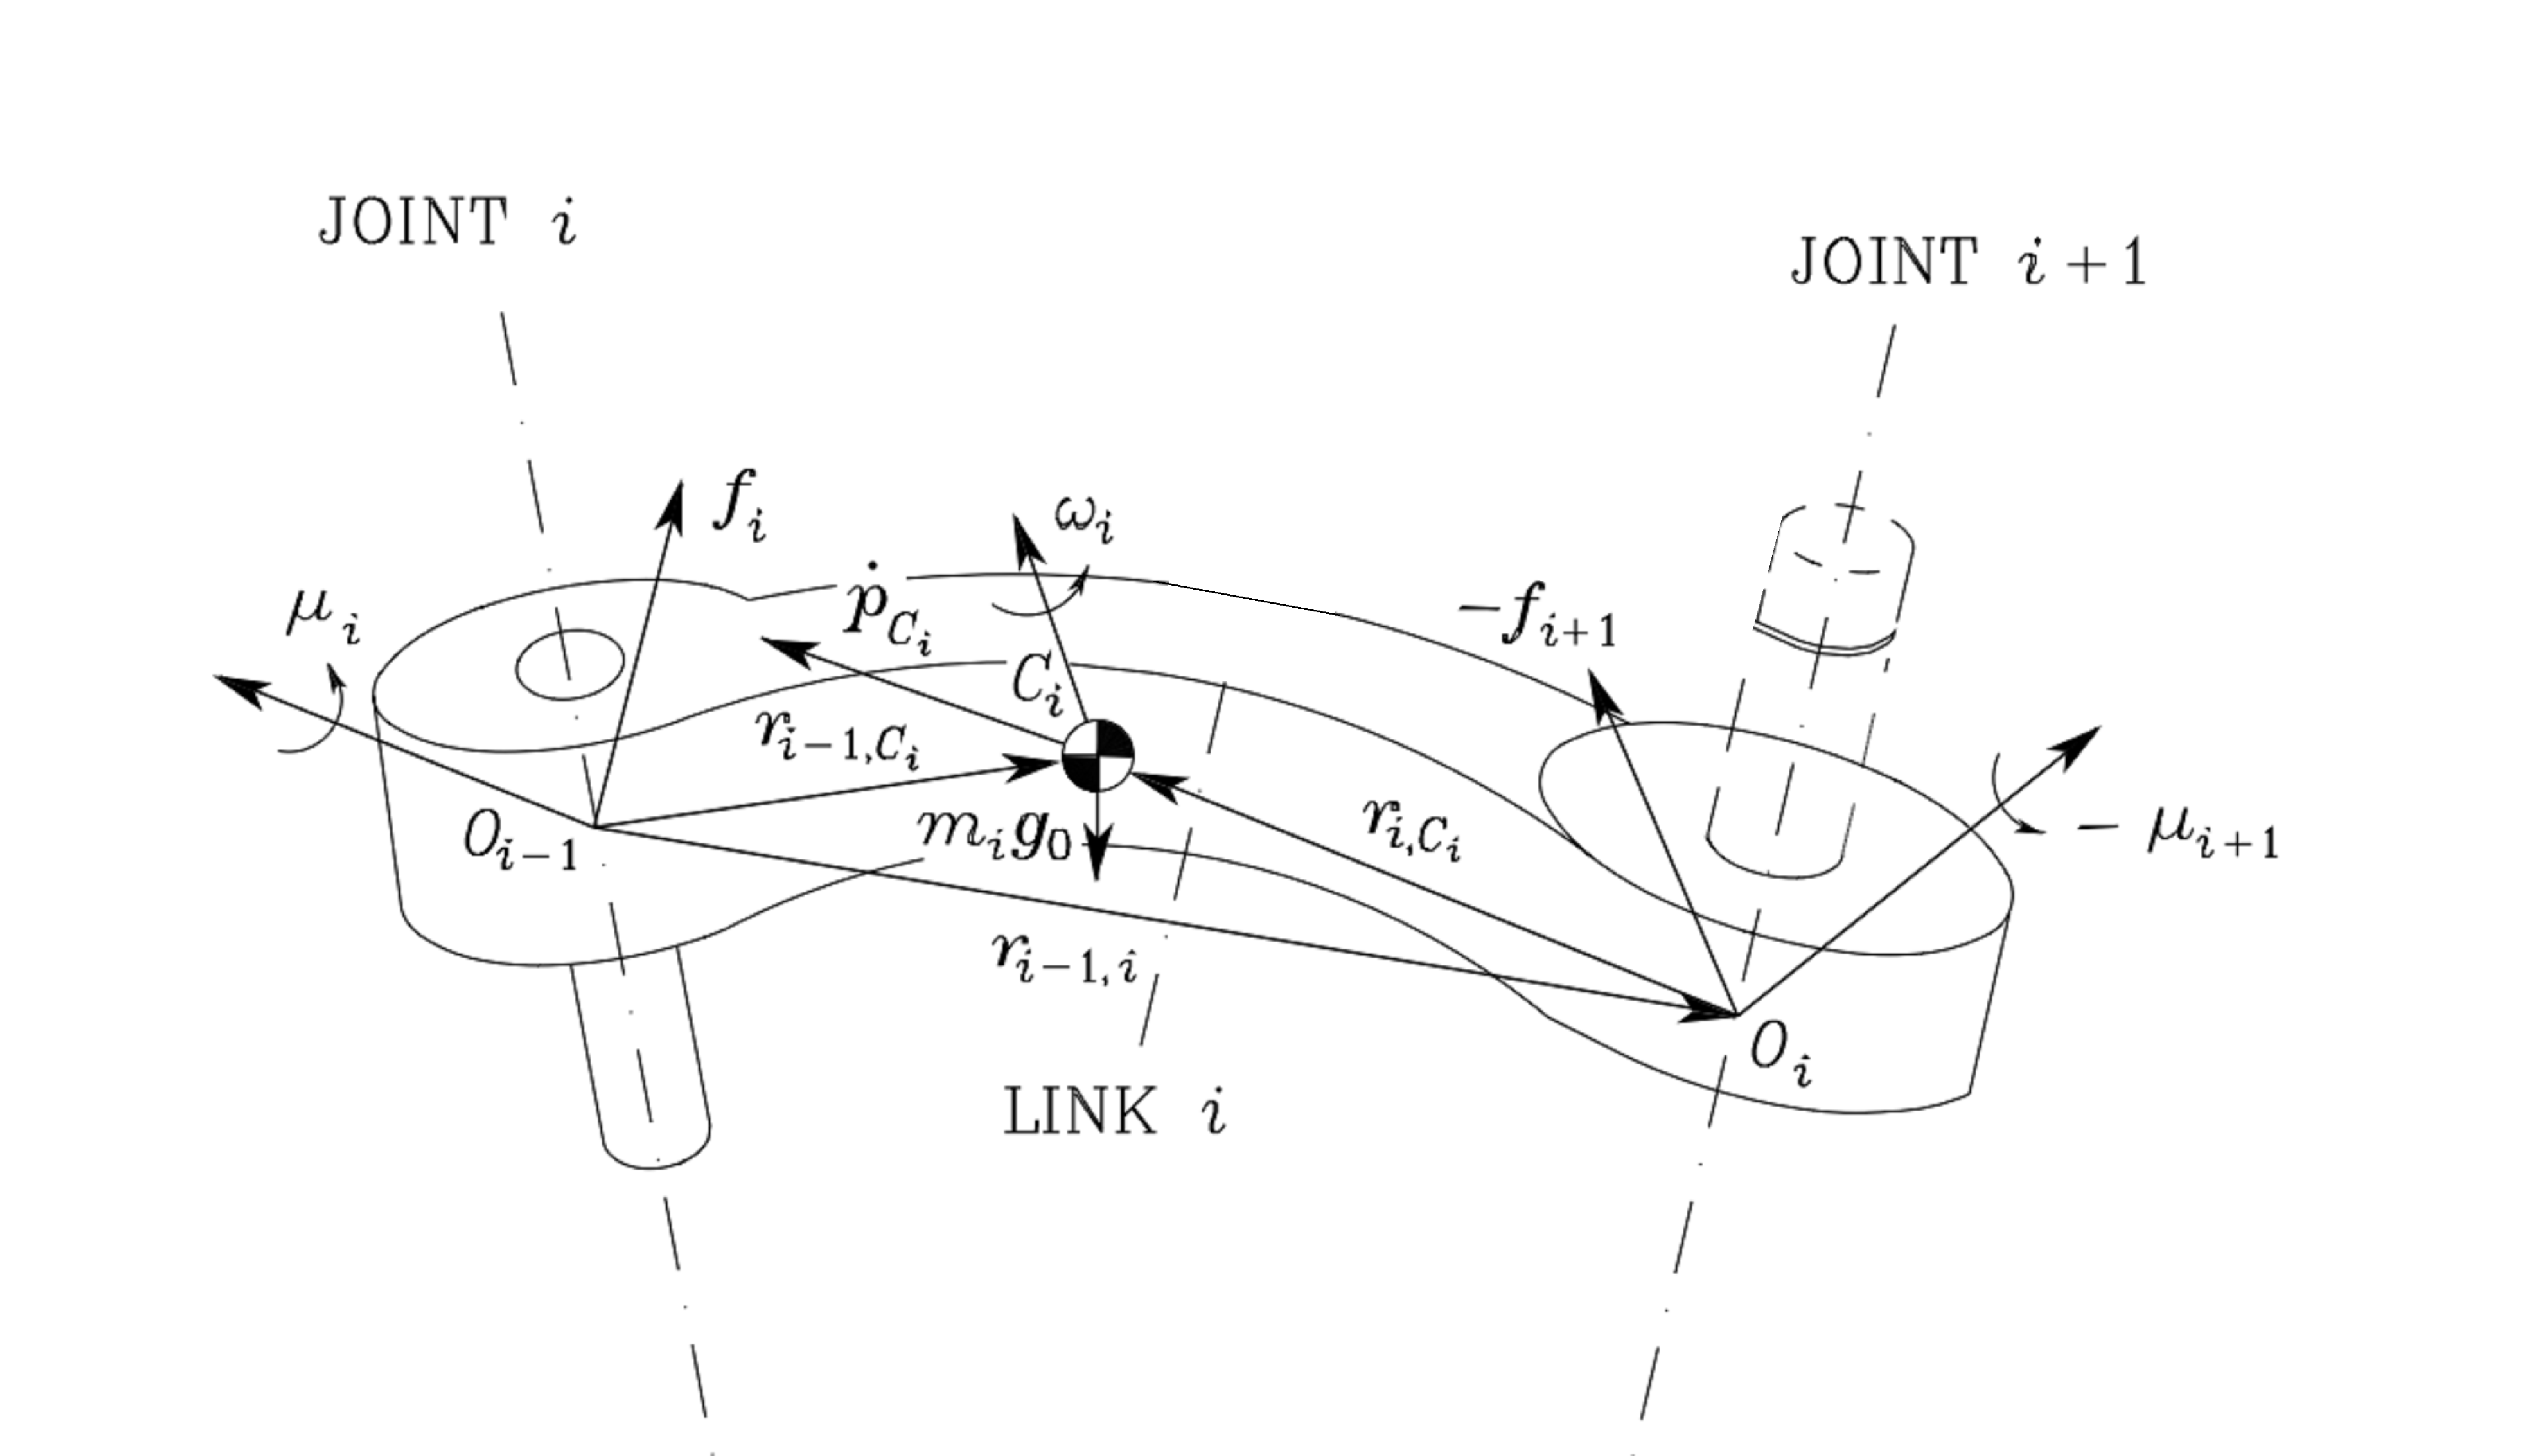
\includegraphics[width=1\linewidth]{images/rnea}
	\caption{generisches Verbindungsglied \cite[S.~283]{Grimble.2009}}
	\label{fig:rnea}
\end{figure} 
%
\subsubsection*{Kräfte und Momente}
\setlist{noitemsep}
\begin{itemize}
	\item $ \boldsymbol{f}_i $ - Kraft, die vom Verbindungsglied $ i-1 $ auf das Verbindungsglied $ i $ ausgeübt wird
	\item $ -\boldsymbol{f}_{i+1} $ - Kraft, die vom Verbindungsglied $ i+1 $ auf das Verbindungsglied $ i $ ausgeübt wird
	\item $ \boldsymbol{\mu}_i $ - Drehmoment, welches vom Verbindungsglied $ i-1 $ auf das Verbindungsglied $ i $ im KS$\left\{i-1\right\}$ des dazugehörigen Gelenks $i$ ausgeübt wird
	\item $ -\boldsymbol{\mu}_{i+1} $ - Drehmoment, welches vom Verbindungsglied $ i+1 $ auf das Verbindungsglied $ i $ im KS$\left\{i\right\}$ des dazugehörigen Gelenks $i+1$ ausgeübt wird
\end{itemize}
%
Die Implementierung des RNEA sieht vor, alle Größen bezogen auf das KS$\left\{i\right\}$ des fest damit verbundenen Verbindungsglieds $i$ zu beziehen. Daraus resultieren die Kräfte und Momente mit der Notation $ \boldsymbol{f}_{i}^{i} $ und $ \boldsymbol{\mu}_i^{i} $. Nachfolgend werden die Parameter der Verbindungsglieder eingeführt. Alle Vektoren beziehen sich ebenfalls auf das KS$\left\{i\right\}$, sodass die Parameter als Konstante weiterverarbeitet werden können. Die Werte der Systemparameter sind im Anhang \ref{add:Systemparameterdef} aufgeführt.
%
\subsubsection*{Parameter}
\setlist{noitemsep}
\begin{itemize}
	\item $ m_i $ - Masse des Verbindungsglieds $i$
	\item $ \bm{I}^{i}_{i} $ - Trägheitstensor des Verbindungsglieds $i$ im fest damit verbundenen KS$\left\{i\right\}$ 
	\item $ \boldsymbol{r}^{i}_{i-1,C_i} $ - Vektor vom Ursprung des KS$\left\{i-1\right\}$ zum Masseschwerpunkt $ C_i $ des Verbindungsglieds $i$ im KS$\left\{i\right\}$ 
	\item $ \boldsymbol{r}^{i}_{i,C_i} $ - Vektor vom Ursprung des KS$\left\{i\right\}$ zum Masseschwerpunkt $ C_i $ im KS$\left\{i\right\}$ 
	\item $ \boldsymbol{r}^{i}_{i-1,i} $ - Vektor vom Ursprung des KS$\left\{i-1\right\}$ zum Ursprung des  KS$\left\{i\right\}$ im KS$\left\{i\right\}$ 
	\item $ i_i$ - Übersetzungsverhältnis der Getriebe
\end{itemize}
%
\subsubsection*{Geschwindigkeiten und Beschleunigungen}
\setlist{noitemsep}
\begin{itemize}
	\item $ \dot{\boldsymbol{p}}_{C_i} $ - Lineare Geschwindigkeit im Masseschwerpunkt $ C_i $ 
	\item $ \dot{\boldsymbol{p}}_i $ - Lineare Geschwindigkeit im Ursprung des KS$\left\{i\right\}$
	\item $ \boldsymbol{\omega}_i $ - Winkelgeschwindigkeit des Verbindungsglieds $i$
	\item $ \ddot{\boldsymbol{p}}_{C_i} $ - Lineare Beschleunigung im Masseschwerpunkt $ C_i $
	\item $ \ddot{\boldsymbol{p}}_i $ - Lineare Beschleunigung im Ursprung des KS$\left\{i\right\}$
	\item $ \boldsymbol{\dot{\omega}}_i $ - Winkelbeschleunigung des Verbindungsglieds $i$
\end{itemize}
%
Mit Kenntnis der Größen $\bm{q}, \dot{\bm{q}}, \ddot{\bm{q}}$ aus der Bahnplanung des Roboters und unter Festlegung der Startbedingungen $\bm{\omega}_0 = 0,~ \ddot{\bm{p}_0}-g = [0,0,-9.81]^T,~ \ddot{\bm{\omega}_0} = 0$  erfolgt sukzessive die Berechnung der Geschwindigkeiten und Beschleunigungen für jedes Verbindungsglied des Roboters vom ersten bis zum sechsten. Ein Endeffektor ist am Versuchsroboter nicht verbaut. Die der Literatur  \cite[S.~287~f.]{Grimble.2009} entnommenen Gleichungen \ref{eqn:rnea0}, \ref{eqn:rnea1}, \ref{eqn:rnea2} und  \ref{eqn:rnea3} werden nachfolgend aufgezeigt. Diese gelten ausschließlich für rotatorische Gelenke, da der betrachtete KUKA KR210 R2700-2 eine RRR-Kinematik mit Zentralhand (rotatorische Funktionen Drehen, Nicken, Gieren) aufweist. 
%
\begin{equation}
	\label{eqn:rnea0}
	\bm{\omega}^i_i = {\bm{R}^{i-1}_i}^T  \left( \bm{\omega}^{i-1}_{i-1} +\dot{\theta}_i\bm{z_0} \right)
\end{equation}
%
\begin{equation}
	\label{eqn:rnea1}
	\dot{\bm{\omega}}^i_i = {\bm{R}^{i-1}_i}^T  \left( \dot{\bm{\omega}}^{i-1}_{i-1} +\ddot{\theta}_i\bm{z_0} +\dot{{\theta}}_i\bm{\omega}^{i-1}_{i-1} \times \bm{z}_0 \right)
\end{equation}
%
\begin{equation}
	\label{eqn:rnea2}
	\ddot{\bm{p}}^i_i = {\bm{R}^{i-1}_i}^T  \ddot{\bm{p}}^{i-1}_{i-1} + \dot{\bm{\omega}}^{i}_{i} \times \bm{r}^{i}_{i-1,i} + {\bm{\omega}}^{i}_{i} \times \left(  {\bm{\omega}}^{i}_{i} \times \bm{r}^{i}_{i-1,i} \right)
\end{equation}
%
\begin{equation}
	\label{eqn:rnea3}
	\ddot{\bm{p}}^i_{C_i} = \ddot{\bm{p}}^{i}_{i} + \dot{\bm{\omega}}^{i}_{i} \times \bm{r}^{i}_{i,C_i} + {\bm{\omega}}^{i}_{i} \times \left(  {\bm{\omega}}^{i}_{i} \times \bm{r}^{i}_{i,C_i} \right)
\end{equation}
%
Im nächsten Schritt erfolgt die rekursive Berechnung der Kräfte und Drehmomente. Der Algorithmus beginnt mit der Berechnung der Größen für das sechste Gelenk, gemäß der Gleichungen \ref{eqn:rnea4}, \ref{eqn:rnea5} und \ref{eqn:rnea6}. $\bm{f}^{n+1}_{n+1}$ und $\bm{\mu}^{n+1}_{n+1}$ werden zu 0 angenommen. 
%
\begin{equation}
	\label{eqn:rnea4}
	\bm{f}^{i}_{i} = \bm{R}^{i}_{i+1} \bm{f}^{i+1}_{i+1} + m_i\ddot{\bm{p}}^{i}_{C_i}
\end{equation}
%
\begin{equation}
	\label{eqn:rnea5}
	\bm{\mu}^{i}_{i} = -\bm{f}^{i}_{i} \times \left( \bm{r}^{i}_{i-1,i} + \bm{r}^{i}_{i,C_i} \right) + \bm{R}^{i}_{i+1} \bm{\mu}^{i+1}_{i+1} + \bm{R}^{i}_{i+1} \bm{f}^{i+1}_{i+1} \times \bm{r}^{i}_{i,C_i} + \bm{I}^{i}_{i} \dot{\bm{\omega}}^{i}_{i} + {\bm{\omega}}^{i}_{i} \times (\bm{I}^{i}_{i}{\bm{\omega}}^{i}_{i})
\end{equation}
%%
\begin{equation}
	\label{eqn:rnea6}
	\tau_i = i_i{\bm{\mu}^{i}_{i}}^T {\bm{R}^{i-1}_{i}}^T [0~0~1]^T
\end{equation}
%
Aufgrund der Lagerausführung des ersten Gelenks wird angenommen, dass das nachfolgende Drehmoment nicht auf das erste Gelenk übertragen wird, sodass der Term $\bm{R}^{i}_{i+1} \bm{\mu}^{i+1}_{i+1}$ hierbei entfällt. Aus der den identifizierten Drehmomenten $\tau_i$ erfolgt durch Multiplikation mit den Winkelgeschwindigkeiten $\dot{{d}}$ die Berechnung der mechanischen Leistung $P_{mech,i}$ Die Implementierung des Modells ist dem Anhang \ref{add:rnea} zu entnehmen. \cite[S.~282~ff.]{Grimble.2009}
%
\section{Annahmen und Vernachlässigungen}
Bei der Entwicklung des mechanischen Modells zur Simulation der Roboterdynamik wurden Annahmen getroffen und Komponenten vernachlässigt, um den Modellierungsaufwand zu reduzieren. Ein wesentlicher Einfluss wird der Vernachlässigung des hydraulischen Gewichtsausgleichs am zweiten Gelenk zugeschrieben. Der Gewichtsausgleich ist aus einem Hydraulikzylinder mit Membranspeicher aufgebaut und wirkt dem am zweiten Gelenk auftretenden Drehmoment entgegen. Im Modell wurde dieser aufgrund fehlender Konstruktionsdaten zu Kolbendurchmesser und Kolbenstangendurchmesser nicht berücksichtigt. Fehlende Daten sind auch der Grund für die Auslassung des Gewichts und der Steifigkeit der Schlauchpakete. Das Gewicht der Elektromotoren (Statorseite) wurde aufgrund fehlender Informationen aus der Verschiebung der Massenschwerpunkte der Achsen vernachlässigt. Aufgrund des Verhältnisses zwischen der Masse der Motoren (Statorseite) und dem Gewicht der Achsen  wird diese Vernachlässigung toleriert. Am Beispiel des dritten Verbindungsglieds beträgt dieses mindesten 1:15. Genaue Daten wie viel Gewicht der Rotor bzw. der Stator einnehmen liegen nicht vor.  Die gleiche Schlussfolgerung gilt für die Massenträgheit der Motoren (Rotorseite) und die daraus resultierenden Momente. \cite[S.~287~f.]{Grimble.2009} berücksichtigt bei der Berechnung der Drehmomente die Einflüsse der viskosen und der coloumbschen Reibung. Die entsprechenden Koeffizienten wurden nicht ermittelt, so dass dieser Einfluss ebenfalls als Vernachlässigung festgehalten wird. Neben der Berechnung der mechanisch aufzuwendenden Leistung erfordert eine hohe Modellgenauigkeit die Berücksichtigung der elektrischen Komponenten in Abbildung \ref{fig:zk}. Bei den Motoren handelt es sich um dreiphasige permanenterregte Synchronmaschinen (PMSM).  Die Steuerung erfolgt über Frequenzumrichter. Im Ersatzschaltbild (ESB) sind alle Antriebe über einen gemeinsamen Gleichrichter vom Netz auf einen Gleichspannungszwischenkreis gekoppelt. PMSM können sowohl motorisch als auch generatorisch betrieben werden. Für die Berechnung des Energieverbrauchs wird angenommen, dass die generatorisch umgewandelte Energie über einen Bremswiderstand als Wärme abgeführt wird. Von einer Spannungs-Schwellwert gesteuerten Zu- und Abschaltung des Bremswiderstands wird abgesehen. \cite[S.~21~ff.]{Eggers.2019}
%
\begin{figure}[tbph]
	\centering
	\includegraphics[width=1\linewidth]{images/zk}
	\caption{Ersatzschaltbild der aufgenommenen Netzleistung \cite[S.~20]{Eggers.2019}}
	\label{fig:zk}
\end{figure}